\section{Data}
This paper employs a dataset of Spanish business news articles sourced from Dow Jones Newswires, covering the period from June 24, 2020, to September 30, 2021. The selection of this timeframe is deliberate, driven by two key considerations. 
%
First, given the substantial computational demands of LLM-based analysis, we strategically focus on a smaller, carefully curated dataset. This deliberate scope reduction allows us to thoroughly demonstrate our novel methodology's effectiveness in decoding market-news relationships while keeping computational costs manageable. 
%Rather than pursuing a broad-scale analysis, we prioritize proving our approach's utility through a focused, computationally feasible study that can serve as a foundation for future expansions.
%
Second, we specifically chose the Covid-19 era to test our methodology's extrapolative capabilities during periods of significant market instability and volatility. While existing textual algorithms typically perform well in stable market conditions, they often struggle to generalize effectively during periods of heightened uncertainty. By focusing on this volatile period, we can better assess our methodology's robustness and its ability to maintain predictive power under challenging market conditions.

The dataset consists of high-quality articles that have been filtered to include only those mentioning Spanish publicly traded firms listed on the IBEX-35 index. These 35 companies represent the largest firms in Spain by market capitalization and are typically the most liquid and actively traded Spanish stocks. Moreover, these companies tend to receive the most consistent media coverage, making them ideal for the scope of our analysis. 

The use of Dow Jones Newswires as our news source is also intentional. Dow Jones has a standard practice of including the stock market ticker of firms directly affected by the article in parentheses, while excluding firms mentioned for secondary purposes from ticker specification.
This feature significantly facilitates the extraction of named entities (i.e., Named Entity Recognition, or NER). The tickers used by Dow Jones align with those from Yahoo Finance, enabling seamless integration between our NER algorithm and subsequent firm-specific trading operations via the Yahoo Finance API.
%
We employ a pattern recognition algorithm through the \texttt{regex} library in Python to identify specific mentions of publicly traded companies in the Spanish stock exchange. The algorithm searches for patterns of the form ``\texttt{(<WORD>.MC)}'' for any \texttt{<WORD>}. For instance, consider the following example article (translated into English for convenience):

\newpage 
\begin{news}
[An article about ACS and Acciona (translated into English)]
[news:article-acs-acciona]
{ACS and Acciona Secure Contracts for New Australian Airport 
}
A consortium of Actividades de Construcci�n y Servicios SA \red{(ACS.MC)} and Acciona SA \red{(ANA.MC)} has won a contract to build the operations area of the Western Sydney International Airport (Nancy-Bird Walton) and carry out paving works, amounting to AUD265 million (EUR164 million) for the Australian subsidiary CIMIC Group Ltd (CIM.AU). CIMIC will carry out the work through its subsidiary CPB Contractors, as stated in a press release. This is the third project awarded by Western Sydney Airport to the joint venture after being selected to carry out earthworks.
Construction will take two years, and the Western Sydney airport is expected to open in 2026.	
\end{news}



Our NER algorithm applied to  Example \ref{news:article-acs-acciona} successfully identifies the Spanish firms \texttt{ACS.MC} (Actividades de Construcci�n y Servicios SA) and \texttt{ANA.MC} (Acciona SA) while disregarding the Australian \texttt{CIM.AU} (CIMIC Groups Ltd). 
To further ensure the reliability of firm identification, we validate the extracted entities using a Large Language Model (LLM).
In particular, we feed the articles to the LLM, which parses them according to a predefined schema. As we will see later, the first task in this schema 
is to identify the listed Spanish firms directly affected by the events described in the article. Finally, the identified firms are filtered against a dynamic list of IBEX-35 members.
Due to the high quality of the dataset, the correlation between entities identified by the LLM and those extracted via pattern recognition is almost exact.

For subsequent analysis, we partition the dataset into three splits: \textit{Train}, \textit{Validation}, and \textit{Test}. Each split serves a distinct purpose that will be explained in detail as we progress through the paper. Summary statistics for each data split are provided in \cref{tab:Articles_Summary_Statistics}.

%----------------------------------------------------
\inserthere{tab:Articles_Summary_Statistics}

\begin{table}[H]
\centering
\caption{Summary Statistics of Articles by Data Split}
\label{tab:Articles_Summary_Statistics}
%\begin{tabular}{|l||c|c|c|c|}
\begin{tabular}{lcccc}
\hline \Xhline{2\arrayrulewidth}
%\rowcolor{gray!10}
\textbf{Data Split} & \textbf{Time Period} & \textbf{\# Articles} & \textbf{\# Words} & \textbf{Vocabulary Size} \\
\hline \Xhline{2\arrayrulewidth}
Train & 24/06/2020 $-$ 12/02/2021 & 1254 & 327413 & 26762 \\
Validation & 12/02/2021 $-$ 21/06/2021 & 836 & 232912 & 22265 \\
Test & 21/06/2021 $-$ 30/09/2021 & 523 & 140495 & 16474 \\ \hline \Xhline{\arrayrulewidth}
All & 24/06/2020 $-$ 30/09/2021 & 2613 & 700820 & 42603 \\ \hline \Xhline{2\arrayrulewidth}
\end{tabular}
\mx 
\subcaption*{\textit{Note: Summary statistics by data splits and for the whole sample. We provide the period spanned by each data split, the number of articles, the number of words, and the vocabulary size. Articles have been preprocessed following standard NLP practices.}}
\end{table}

%----------------------------------------------------

The most frequently used words in the whole dataset are depicted in \cref{fig:WordCloud} by means of a WordCloud. As shown, the most prominent words include \qquote{empresa} (firm), \qquote{compa��a} (company), and \qquote{espa�a} (Spain), reinforcing that the dataset primarily comprises Spanish business news, with a prevalence of technical terms such as \qquote{beneficio neto} (net profit), \qquote{precio objetivo} (target price), \qquote{proyecto} (project), and \qquote{operaci�n} (operation).

%----------------------------------------------------
\inserthere{fig:WordCloud}
\begin{figure}[H]
  \centering
  \caption{Word Cloud of all the dataset}
  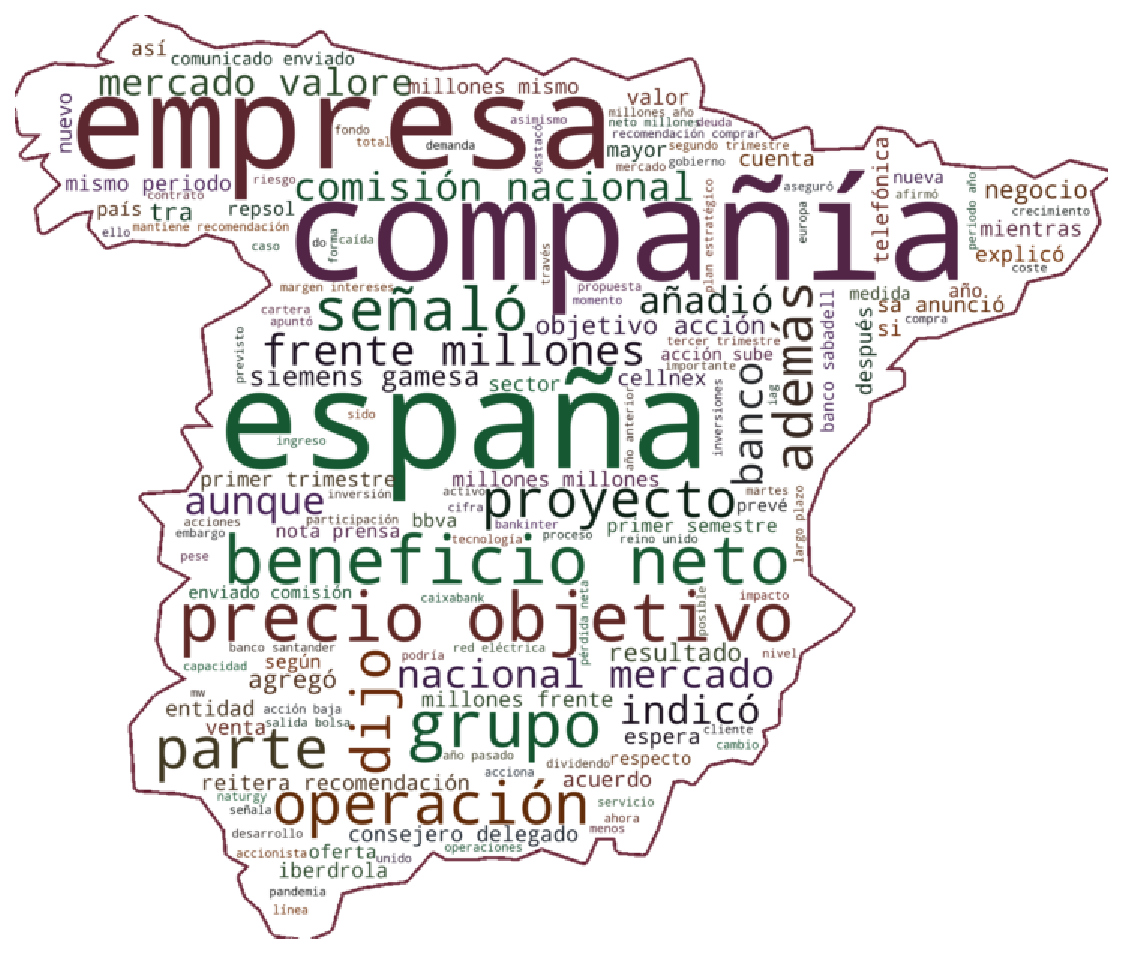
\includegraphics[scale=0.496]{fig_1_EDA_WordCloud.pdf}
  \label{fig:WordCloud}
  \subcaption*{\textit{Note: This Word Cloud visualizes the most frequent words in our dataset of Spanish business news articles. Larger words correspond to higher frequencies. The color of the words is purely for visual differentiation and holds no additional meaning. The most prominent words include \qquote{empresa} (firm), \qquote{compa��a} (company), and \qquote{espa�a} (Spain), reinforcing that the dataset primarily comprises Spanish business news, with a prevalence of technical terms such as \qquote{beneficio neto} (net profit), \qquote{precio objetivo} (target price), \qquote{proyecto} (project), and \qquote{operaci�n} (operation).}}
\end{figure}
%----------------------------------------------------

The distribution of the number of articles published per day is illustrated in \cref{fig:hist_1}, showing that the most frequent publication rate is between 5 and 10 articles per day, though some days exhibit unusually high publication counts. \cref{fig:hist_2} shows the distribution of the number of words per article, with the majority of articles containing between 70 and 280 words. This indicates that the articles are relatively succinct, providing direct information. 
However, the long right tail points to instances of more comprehensive coverage.

%----------------------------------------------------
\inserthere{fig:histograms}
\begin{figure}[H]
  \caption{Histogram of \# News Articles per Day and \# Words per Article}
  \centering
  \begin{subfigure}[b]{0.46\textwidth}
    \centering
    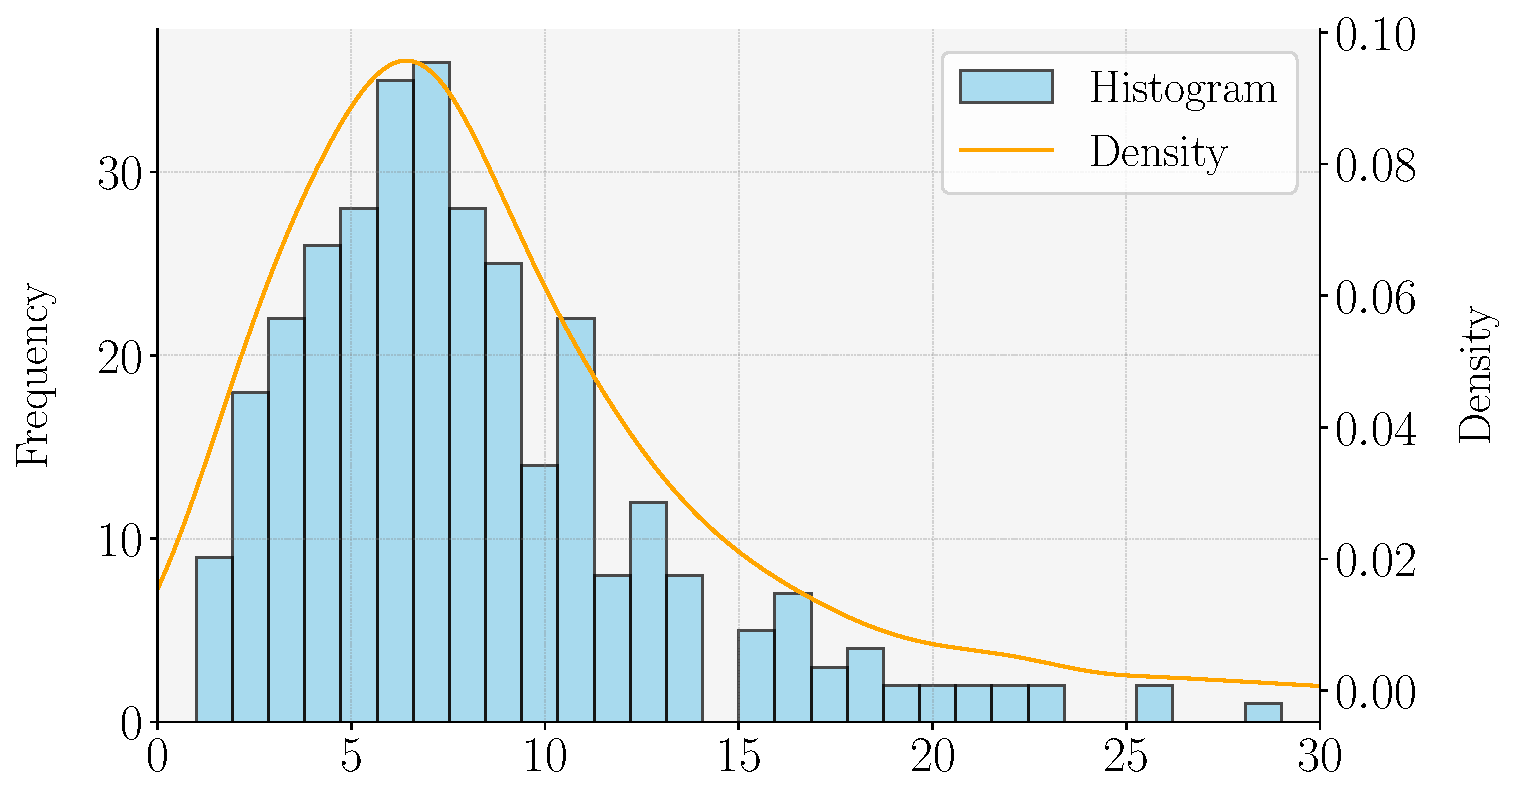
\includegraphics[width=\textwidth]{fig_2a_EDA_News_Articles_per_day.pdf}
    \caption{Number of News Articles per Day}
    \label{fig:hist_1}
  \end{subfigure}
  \hspace{0.05\textwidth} % Add horizontal space between the subfigures
  \begin{subfigure}[b]{0.46\textwidth}
    \centering
    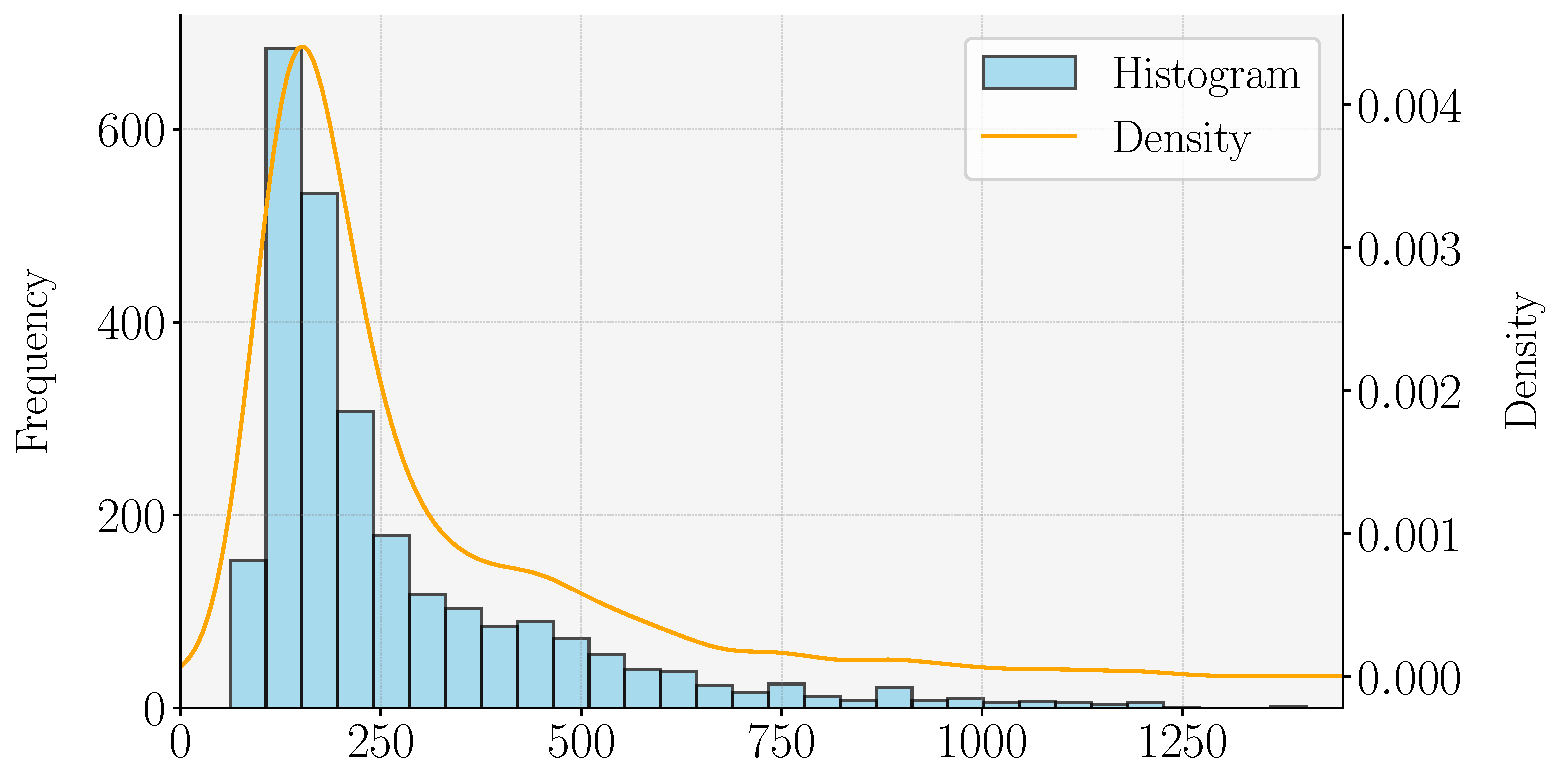
\includegraphics[width=\textwidth]{fig_2b_EDA_Words_per_Article.pdf}
    \caption{Number of Words per Article}
    \label{fig:hist_2}
  \end{subfigure}
  \label{fig:histograms}
  \subcaption*{\textit{Note: Panel (a) displays the distribution of the number of news articles published per day, with most days having between 5 and 10 articles. Panel (b) shows the distribution of the number of words per article, where the majority are between 70 and 280 words, suggesting concise reporting. However, the long right tail indicates instances of more comprehensive coverage.}}

\end{figure}
%----------------------------------------------------

The time series of the number of articles published per day throughout the sample period is shown in \Cref{fig:ts_articles}. The series exhibits considerable variability, with frequent fluctuations from fewer than 5 articles per day to sudden spikes exceeding 20 articles. The 30-day moving average smooths the series, confirming the previous observation that, on average, between 5 and 10 articles are published daily.

%----------------------------------------------------
\inserthere{fig:ts_articles}
\begin{figure}[H]
  \centering
  \caption{Time Series of Number of Articles per Day and 30-Period Moving Average}
  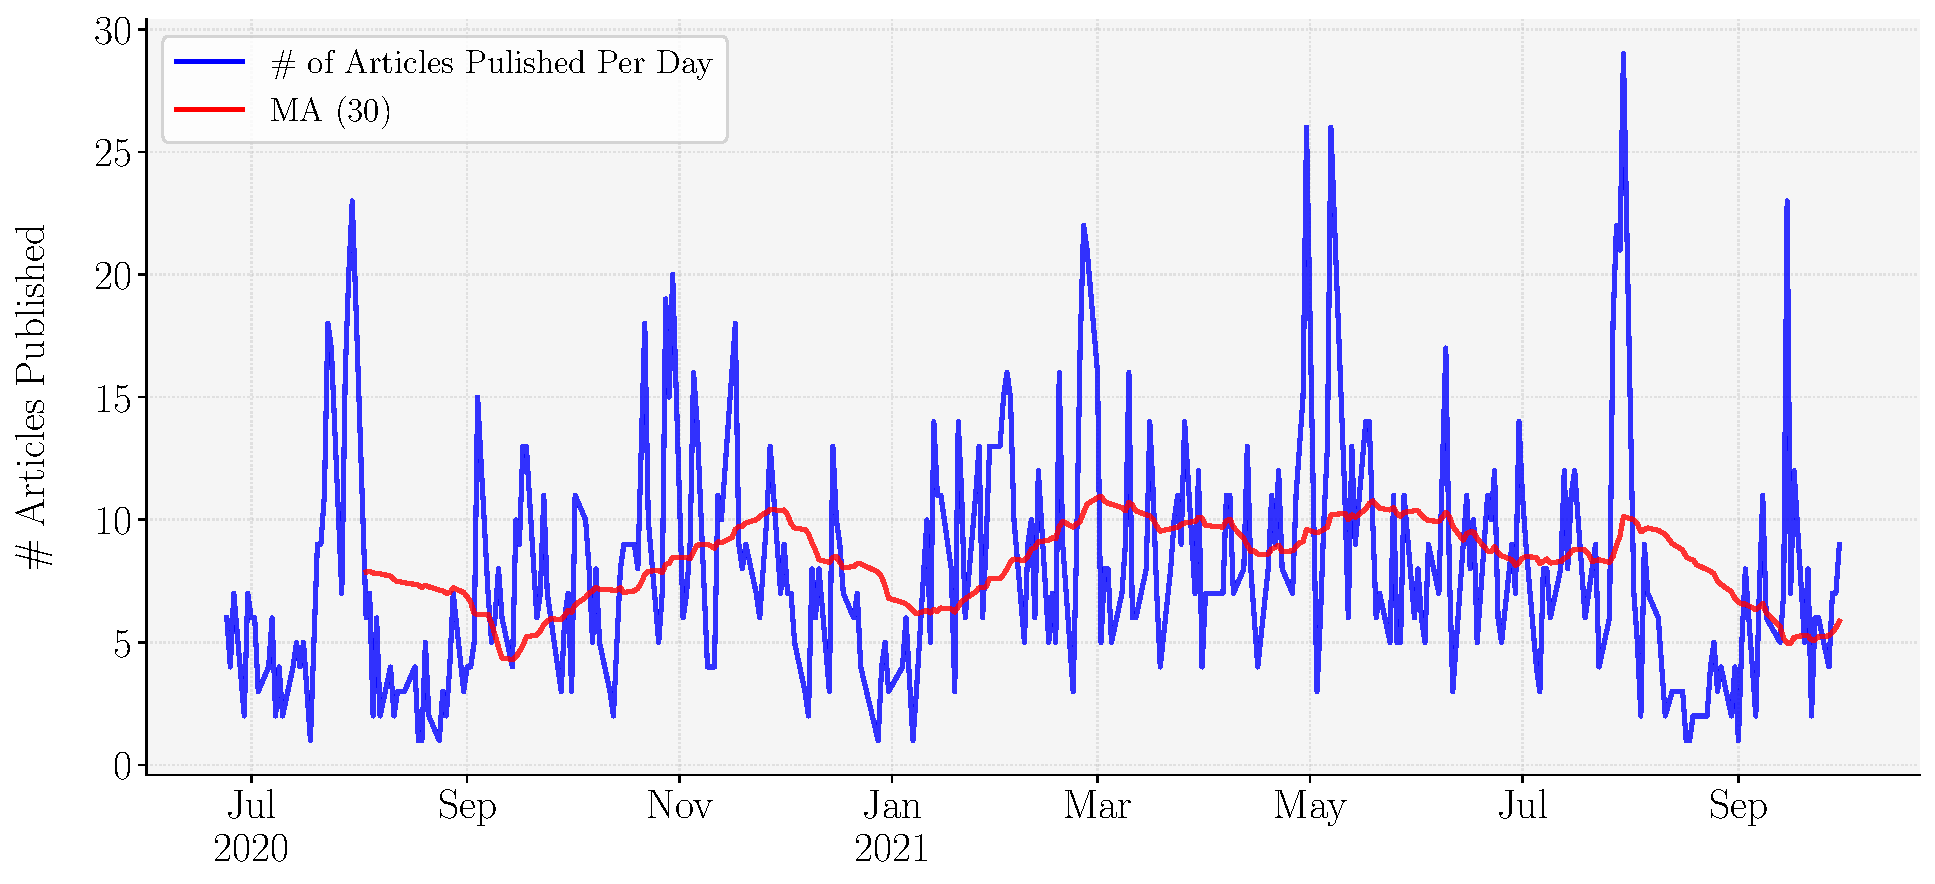
\includegraphics[scale=0.445]{fig_3_EDA_Time_Series_of_Articles.pdf}
  \label{fig:ts_articles}
  \subcaption*{\textit{Note: The time series shows the daily number of news articles published, characterized by significant variability with occasional sharp spikes. The 30-day moving average smooths these fluctuations, revealing an average publication rate of 5 to 10 articles per day.}}
\end{figure}
%----------------------------------------------------


\textbf{Data Availability.} 
% OPTION 1
The dataset used in this study contains confidential information provided under agreements with the Bank of Spain and Dow Jones Newswires, and cannot be shared publicly or with third parties. Interested readers may access the same data from Dow Jones Newswires for a fee.
%We are committed to transparency in our research methods and are available to discuss our methodology and provide additional non-confidential details upon request.
% OPTION 2
%Due to confidentiality and proprietary constraints, the dataset used in this research is not publicly available. Any inquiries regarding the data availability should be directed to the relevant parties who own the data.

